%---------- COURSE INFORMATION ------------------------
\newcommand{\course}{CS 366-02}
\newcommand{\coursetitle}{DATABASE DEVELOPMENT AND MANAGEMENT}
\newcommand{\courseloc}{Raburn 211}
\newcommand{\coursetime}{Tuesday/Thursday 11:00 a.m. - 12:15 p.m.}
\newcommand{\coursedesc}{An introduction to the theory and practice of database design and processing within the
	information systems (IS) framework. This includes fundamental design concepts, technical aspects, and components of
	relational databases and database management systems (DBMS), and use of	specific DBMS software. Emphasis is placed
	on the importance of the management and	effective use of the data resource within an organization.}
\newcommand{\coursesec}{02}
\newcommand{\coursecredithours}{3}
\newcommand{\courseprereq}{CIS 225, 236	(with a grade of ``C'' or higher in both)}
\newcommand{\coursedelmethod}{Traditional Classroom}

\newcommand{\courseobjectives}{
	\item Gain an understanding of the role of database management systems in organizations [CIS Program Outcome a].
	\item Develop an introductory understanding of relational database principles, design, technology, and applications including [CIS Program Outcomes a,b,i]:
	\begin{enumerate}
	  \item Entity Relationship Diagraming
	  \item Structured Query Language (SQL)
	  \item Normalization
    \end{enumerate}
	\item Learn skills required to develop database systems that may be used to	support organizational data collection, analysis, and reporting [CIS Program Outcomes a,b,c,i].
	\item Learn to communicate and work in teams [CIS Program Outcome d].
	\item Learn the need for engaging in continuing professional development [CIS Outcome h].
}

\newcommand{\coursetopics}{
\item Introduction to database \& database development
\item Modeling data in the organization
\item Logical database design and the relational model
\item Physical database design and performance
\item Introduction to SQL
\item Database application development
\item Overview of data warehousing / data mining
}
\newcommand{\coursegrades}{
	Subject Exams (3 exams @ 20\% each)\dotfillsmall 60\% \\
	Projects and other assignments\dotfillsmall 40\% 
}
\newcommand{\coursetext}{\adjustbox{valign=c}{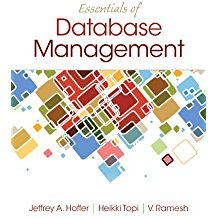
\includegraphics[width=1in]{img/cis366}} & \hangindent .4in \textbf{Textbook:} Essentials of Database Management. Jeffrey A. Hoffer Heikki Topi Ramesh Venkataraman. ISBN-10: 0133405680 $\bullet$ ISBN-13: 9780133405682  \\
	%& \hangindent .4in Simulation Software: SAM 365 \& 2016 Assessments, Trainings, and Projects with MindTap Reader.
}